%LTeX: language=DE
\chapter{Vorbereitung}
	Im Praktikumsversuch wird das Verhalten eines Step-Down Reglers mit der Bezeichnung \textit{LM2596-5.0} untersucht.
	Als Referenz wird das Datenblatt zur Bauteilreihe \textit{LM2596} von \textsc{Texas Instruments} verwendet \cite{datasheet.LM2596.TexasInstruments.2021}.\par
	Dieses Bauteil ist nicht in der Standardbibliothek von dem im Praktikum benutzten Simulationsprogramm \textsc{LTSpice} vorhanden.
	Um es anzulegen, wird die von \textsc{Texas Instruments} bereitgestellte Bibliotheksdatei -- zu erreichen unter \url{https://www.ti.com/lit/zip/snvma62} --
	verwendet.\par\medskip
	\Cref{fig:basisschaltung} zeigt die Beschaltung um das zentrale Bauteil gemäß der in Kapitel 1 des Datenblattes zu findenden \textit{Typical Application}.
	\begin{figure}[h]
		\centering
		% \includesvg[inkscapelatex=false, width=.8\textwidth]{LTSpice/figures/basis_schematic_LM2596}
		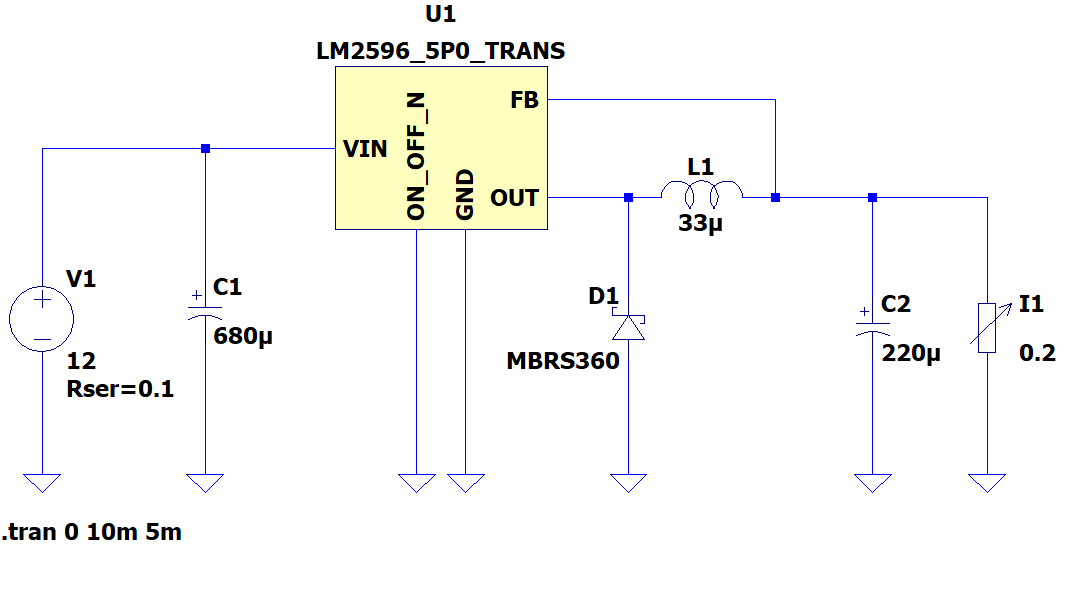
\includegraphics[width=.8\textwidth]{LTSpice/figures/basis_schematic_LM2596.png}
		\caption[Basisschaltung des \textit{LM2596}]{Basisschaltung des \textit{LM2596} gemäß \textit{Typical Application} in Kapitel 1 des Datenblatts \cite{datasheet.LM2596.TexasInstruments.2021}.}
		\label{fig:basisschaltung}
	\end{figure}
